\section{The framework}
\label{sec:framework}

The work of this thesis is designated as ``a front-end for LISA''. The term ``front-end'' is generally used for layered architectures to outline a layer that is the closest to the user. Often this corresponds to some kind of interface, though what is understood as a user and an interface can vary depending on the context. In our case, we understand front-end as a programmatic interface for the end-user of LISA. More precisely, we were interested in designing a framework that depended on the LISA kernel and strove to provide a higher-level interface to develop proofs. The use of an indefinite article in our designation is to emphasize the fact that such a layer is by essence guided by opinionated design choices.

One could wonder about the necessity of relying on an existing system. The fundamental reason is to keep the core of the system sufficiently small and simple enough that it could be understood, reasoned about and perhaps formally proved by another system. We refer to this part as the \textbf{kernel} of LISA. The constraint on the complexity of the kernel gives us better reasons to trust its correctness. On the other side, the front-end does not make such claims and can thus be made arbitrarily more sophisticated. The only requirement is for the front-end to be able to reconstruct all of its proofs in the kernel, such that one could check them with the same level of confidence as if they were initially written there. We define soundness as the property for a proof in the front to have the same meaning as one in the kernel, and to be valid there. By the requirement, soundness thus relies on the only assumption that statements in the front are logically equivalent to statements in the kernel. As a consequence such a system would satisfy the De Bruijn criterion, in the sense that the underlying proofs can be checked by a reasonably simple procedure: the kernel.

Another aspect of the front is that despite its dependency on the kernel, it does not expose it to the user. Instead, it redefines most of its components and provides mappings for uni or bi-directional translations. The motivation is two-fold. First of all, it allows us to extend the existing functionality. Practically, for example, it was decided that the kernel would not provide schematic connectors as they were not strictly needed. However the front requires such a functionality to represent its pattern variables and it is not possible to emulate them at low cost. Consequently we implement this functionality in the front and provide conversions. We can also strengthen some of the kernel features, for instance by representing sequents as indexed sequences rather than sets. We may additionally redefine the method \code{toString} on all of our classes. Secondly, it allows us to enrich the language and bring type safety guarantees. Some types in the kernel are (purposely) weak and require runtime checks to ensure safety. This aspect contributes to building a strong framework and is compatible with the mid-term objective of having LISA exist as a Scala library.

\begin{figure}[H]
  \centering
  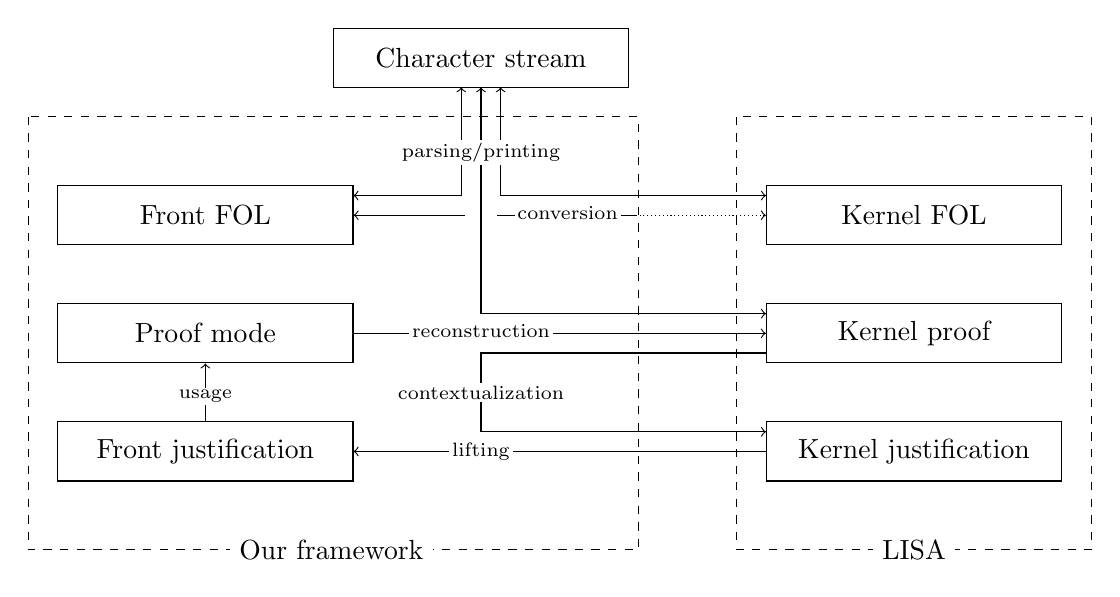
\begin{tikzpicture}[box/.style = {draw, rectangle, minimum width=3.75cm, minimum height=0.75cm}, group/.style = {draw, rectangle, dashed}, label/.style = {fill=white, inner sep=1,outer sep=1}]
  \node[box, minimum width=3.75cm] at (-1, 2) (string) {Character stream};
  \node[box] at (-4.5, 0) (front-fol) {Front FOL};
  \node[box] at (4.5, 0) (kernel-fol) {Kernel FOL};
  \node[box] at (-4.5, -1.5) (front-proof-mode) {Proof mode};
  \node[box] at (4.5, -1.5) (kernel-proof) {Kernel proof};
  \node[box] at (-4.5, -3) (front-justification) {Front justification};
  \node[box] at (4.5, -3) (kernel-justification) {Kernel justification};
  \draw[group] (-6.75, 1.25) rectangle (1, -4.25);
  \draw[group] (2.25, 1.25) rectangle (6.75, -4.25);
  \draw[<-] (front-fol.east) -- ++(3.6, 0);
  \draw[<-, densely dotted] (kernel-fol.west) -- ++(-1.6, 0);
  \draw[<->] (-2.62, 0.25) -| (-1.25, 1.625);
  \draw[<->] (-0.75, 1.625) |- (2.62, 0.25);
  \path[label] (-1.2, 0.2) rectangle (-0.8, -0.2);
  \draw[<->] (-1, 1.625) |- (2.62, -1.25);
  \draw[->] (front-proof-mode.east) -- (kernel-proof.west);
  \draw[->] (kernel-justification.west) -- (front-justification.east);
  \draw[<-] (2.62, -2.75) -| (-1, -1.75) -- (2.62, -1.75);
  \draw[->] (front-justification) -- (front-proof-mode);
  \node[label] at (-1, 0.8) (label1) {\scriptsize{parsing/printing}};
  \node[label] at (0.1, 0.03) (label2) {\scriptsize{conversion}};
  \node[label] at (-1, -1.47) (label3) {\scriptsize{reconstruction}};
  \node[label] at (-1, -2.25) (label4) {\scriptsize{contextualization}};
  \node[label] at (-1, -3) (label5) {\scriptsize{lifting}};
  \node[label] at (-4.5, -2.3) (label6) {\scriptsize{usage}};
  \node[fill=white] at (-2.9, -4.25) (label7) {Our framework};
  \node[fill=white] at (4.5, -4.25) (label8) {LISA};
  \end{tikzpicture}
  \caption[Data flow between the front and the kernel]{Illustration of the data flow between the front and the kernel.}
  \label{fig:front-kernel}
\end{figure}

The interaction between the front and the kernel is relatively limited as the front handles its own state independently (\autoref{fig:front-kernel}). The common ground between the two are justified statements (axioms, theorems, definitions), which means that such objects can be converted back and forth. Whenever a theorem is proven in the front, it is translated to the kernel and checked for consistency. The front obtains the mirror of that justified statement and can be quite certain about its correctness. This enables full compatibility with LISA, making it possible to lift theorems that were not proven in the front.

\subsection{Language and tools}

The implementation was done in Scala version 3\footnote{Also known as Dotty: \href{https://dotty.epfl.ch}{dotty.epfl.ch}.}. The choice of version was a requirement, following the decision to upgrade LISA from version 2 to 3. Since this project does not work directly on the LISA codebase but instead depends on it as a library, both versions must be the same. Regarding the version, it turns out that some of the features implemented in this project would not have had an equivalent encoding in the older version, which lets us to confidently argue that Scala version 3 is an appropriate language for the design of DSL\footnote{DSL: domain specific language} libraries.

During the implementation, eight bugs were discovered in different areas of the Dotty compiler. All the issues that could be minimized and reproduced were reported\footnote{
\href{https://github.com/lampepfl/dotty}{github.com/lampepfl/dotty}:
\href{https://github.com/lampepfl/dotty/issues/14667}{\#14667},\
\href{https://github.com/lampepfl/dotty/issues/14707}{\#14707},\
\href{https://github.com/lampepfl/dotty/issues/14765}{\#14765},\
\href{https://github.com/lampepfl/dotty/issues/14818}{\#14818},\
\href{https://github.com/lampepfl/dotty/issues/14834}{\#14834},\
\href{https://github.com/lampepfl/dotty/issues/14858}{\#14858},\
\href{https://github.com/lampepfl/dotty/issues/14907}{\#14907},\
\href{https://github.com/lampepfl/dotty/issues/15145}{\#15145}.
}\textsuperscript{,}\footnote{
\href{https://github.com/scalameta/scalameta}{github.com/scalameta/scalameta}:
\href{https://github.com/scalameta/scalameta/issues/2741}{\#2741}.
}; most of them have since been fixed or are still in the process of getting fixed.

\subsection{Structure}

\begin{figure}[H]
  \centering
  % https://tex.stackexchange.com/q/515582
  \begin{tikzpicture}[grow via three points={one child at (1.0,-0.6) and two children at (1.0,-0.6) and (1.0,-1.2)}, edge from parent path={(\tikzparentnode.south)|-(\tikzchildnode.west)}]
  \node{(root package)}
  child{node{\code{example}}}
  child{node{\code{front}}
      child{node{\code{fol}}}
      child{node{\code{parser}}}
      child{node{\code{printer}}}
      child{node{\code{proof}}}
      child{node{\code{theory}}}}
  child [missing] {}
  child [missing] {}
  child [missing] {}
  child [missing] {}
  child [missing] {}
  child{node{\code{util}}}
  child{node{\code{legacy}}};
  \node at (6, -0.6) {\parbox{7cm}{\hspace*{0pt}\hfill(examples)}};
  \node at (6, -1.2) {\parbox{7cm}{\hspace*{0pt}\hfill(the front-end framework)}};
  \node at (6, -1.8) {\parbox{7cm}{\hspace*{0pt}\hfill(first-order logic)}};
  \node at (6, -2.4) {\parbox{7cm}{\hspace*{0pt}\hfill(FOL parsers)}};
  \node at (6, -3.0) {\parbox{7cm}{\hspace*{0pt}\hfill(FOL and proof printers)}};
  \node at (6, -3.6) {\parbox{7cm}{\hspace*{0pt}\hfill(logic for proofs, depends on FOL)}};
  \node at (6, -4.2) {\parbox{7cm}{\hspace*{0pt}\hfill(available theories)}};
  \node at (6, -4.8) {\parbox{7cm}{\hspace*{0pt}\hfill(utilities that only rely on the kernel)}};
  \node at (6, -5.4) {\parbox{7cm}{\hspace*{0pt}\hfill(older experiments)}};
  \end{tikzpicture}
  \caption[Source code packages structure]{Structure of the packages in the source code. The reader is invited to review the package \code{example}, which contains a collection of examples giving an overview of the framework.}
  \label{fig:packages}
\end{figure}

The code is organized hierarchically to reduce coupling. This is achieved through Scala dependent members: the components are implemented as children of traits, these traits can then extend and mix with other traits to benefit from their features (included the inherited ones). Finally, all the traits are aggregated in a singleton object that acts as a module. All the components can then be put into scope using a single import. Note that if a same member is exported from two distinct modules it will be considered as a different entity: this is because the types are path-dependent.

\subsection{DSL}

Our framework introduces its own DSL\footnote{DSL: Domain-Specific Language, a custom language designed for a particular purpose.} implemented in Scala. In this section we briefly describe it and explain in more details two interesting problems.

% Crow's foot notation on tikz: https://tex.stackexchange.com/a/393568
\tikzset{
  zig zag to/.style={
    to path={(\tikztostart) -| ($(\tikztostart)!#1!(\tikztotarget)$) |- (\tikztotarget) \tikztonodes}
  },
  zig zag to/.default=0.5pt,
  one to many/.style={
    one-many, zig zag to,
  },
  oone to many/.style={
    oone-many, zig zag to,
  },
  oone to nmany/.style={
    oone-nmany, zig zag to,
  },
  one to nmany/.style={
    one-nmany, zig zag to,
  },
}
\pgfarrowsdeclare{many}{many}
{
  \pgfarrowsleftextend{+-.5\pgflinewidth}%
  \pgfarrowsrightextend{+.5\pgflinewidth}%
}
{
  \let\pgfutil@tempdima=0.6pt%
  \pgfsetdash{}{+0pt}%
  \pgfsetmiterjoin%
  \pgfpathmoveto{\pgfqpoint{0pt}{-6pt\pgfutil@tempdima}}%
  \pgfpathlineto{\pgfqpoint{-8pt\pgfutil@tempdima}{0pt}}%
  \pgfpathlineto{\pgfqpoint{0pt}{6pt\pgfutil@tempdima}}%
  \pgfpathmoveto{\pgfqpoint{0pt\pgfutil@tempdima}{0pt\pgfutil@tempdima}}%
  \pgfpathmoveto{\pgfqpoint{-8pt}{-6pt}}% 
  \pgfpathlineto{\pgfqpoint{-8pt}{-6pt}}%  
  \pgfpathlineto{\pgfqpoint{-8pt}{6pt}}% 
  \pgfusepathqstroke%
}
\pgfarrowsdeclare{nmany}{nmany}
{
  \pgfarrowsleftextend{+-.5\pgflinewidth}%
  \pgfarrowsrightextend{+.5\pgflinewidth}%
}
{
  \let\pgfutil@tempdima=0.6pt%
  \pgfsetdash{}{+0pt}%
  \pgfsetmiterjoin%
  \pgfpathmoveto{\pgfqpoint{0pt}{-6pt\pgfutil@tempdima}}%
  \pgfpathlineto{\pgfqpoint{-8pt\pgfutil@tempdima}{0pt}}%
  \pgfpathlineto{\pgfqpoint{0pt}{6pt\pgfutil@tempdima}}%
  \pgfpathmoveto{\pgfqpoint{0pt\pgfutil@tempdima}{0pt\pgfutil@tempdima}}%
  \pgfpathmoveto{\pgfqpoint{-8pt}{-6pt}}% 
  \pgfpathlineto{\pgfqpoint{-8pt}{-6pt}}%  
  %\pgfpathlineto{\pgfqpoint{-8pt}{6pt}}% 
  \pgfusepathqstroke%
}
\pgfarrowsdeclare{one}{one}
{
  \pgfarrowsleftextend{+-.5\pgflinewidth}%
  \pgfarrowsrightextend{+.5\pgflinewidth}%
}
{
  \let\pgfutil@tempdima=0.6pt%
  \pgfsetdash{}{+0pt}%
  \pgfsetmiterjoin%
  \pgfpathmoveto{\pgfqpoint{0pt\pgfutil@tempdima}{0pt\pgfutil@tempdima}}%
  \pgfpathmoveto{\pgfqpoint{-6pt}{-6pt}}% 
  \pgfpathlineto{\pgfqpoint{-6pt}{-6pt}}%  
  \pgfpathlineto{\pgfqpoint{-6pt}{6pt}}% 
  \pgfpathmoveto{\pgfqpoint{0pt\pgfutil@tempdima}{0pt\pgfutil@tempdima}}%
  \pgfpathmoveto{\pgfqpoint{-8pt}{-6pt}}% 
  \pgfpathlineto{\pgfqpoint{-8pt}{-6pt}}%  
  \pgfpathlineto{\pgfqpoint{-8pt}{6pt}}%    
  \pgfusepathqstroke%
}
\pgfarrowsdeclare{oone}{oone}
{
  \pgfarrowsleftextend{+-.5\pgflinewidth}%
  \pgfarrowsrightextend{+.5\pgflinewidth}%
}
{
  \let\pgfutil@tempdima=0.6pt%
  \pgfsetdash{}{+0pt}%
  \pgfsetmiterjoin%
  \pgfpathmoveto{\pgfqpoint{0pt\pgfutil@tempdima}{0pt\pgfutil@tempdima}}%
  \pgfpathmoveto{\pgfqpoint{-4pt}{-6pt}}%  
  \pgfpathlineto{\pgfqpoint{-4pt}{6pt}}% 
  \pgfpathmoveto{\pgfqpoint{0pt\pgfutil@tempdima}{0pt\pgfutil@tempdima}}%
  \pgfpathmoveto{\pgfqpoint{-8pt}{-6pt}}%
  \pgfpathcircle{\pgfpoint{-10pt}{0}} {3.5pt}
  \pgfusepathqstroke%
}
\begin{figure}[H]
  \centering
  \begin{tikzpicture}[auto, on grid, node distance=5cm, block/.style = {draw, fill=white, rectangle, minimum height=1cm, minimum width=2cm}, none/.style = {draw=none}]
  \node [block] (sequent) {\code{Sequent}};
  \node [block, right = of sequent] (formula) {\code{Formula}};
  \node [block, right = of formula] (term) {\code{Term}};
  \node [none] at (2.5, 0.25) {\footnotesize{is made of}};
  \node [none] at (7.5, 0.25) {\footnotesize{can combine}};
  \node [none] at (5, 1.5) {\footnotesize{can combine other}};
  \node [none] at (10, 1.5) {\footnotesize{combines other}};
  \draw [one to nmany] (sequent) -- (formula);
  \draw [oone to nmany] (formula) -- (term);
  \draw [oone to many] (formula.north) ++(-0.6, 0) |- ++(0, 0.75) |- ++(1.2, 0) -| ++(0, -0.75);
  \draw [one to nmany] (term.north) ++(-0.6, 0) |- ++(0, 0.75) |- ++(1.2, 0) -| ++(0, -0.75);
  \end{tikzpicture}
  \caption[First-order logic relationships]{First-order logic relationships presented in \textit{crow's foot} notation. Each relation corresponds to at least one syntactic combinator.}
  \label{fig:fol-erd}
\end{figure}


The major function of the DSL to assist the developer in using the first-order logic package (\autoref{fig:fol-erd}), namely to provide methods to construct objects in an intuitive way. The second aspect is to provide compile-time safety guarantees when doing so. For instance the sequent $\vdash f(a, b), c \land d$ can be written as \code{|- (f(a, b), a /\textbackslash~a)} in our Scala DSL. Scala allows custom infix operators to be defined, therefore the operators of propositional logic are straightforward to implement. The first interesting problem is about converting the tuple \code{(t1:~T1, ..., tn:~TN)} into a sequence of values of type \code{T1 {|} ...~{|} TN}. While tuples have a method to iterate over their members, this solution is unsound because it loses all type information. Instead, we rely on a mechanism offered by the language: \textit{given} instances and conversions (\autoref{lst:generic-tuples-1}).

\begin{lstlisting}[language=Scala,caption={[Generic tuples (1)]{Generic tuples: converting a tuple of \code{T} into a \code{Seq[T]}.}},label={lst:generic-tuples-1}]
trait Converter[R, S] extends (R => Seq[S])

// Tuple: base case
given[S]: Converter[EmptyTuple, S] with {
  def apply(t: EmptyTuple): Seq[S] = Seq()
}
// Tuple: inductive case
given[S, H <: S, T <: Tuple](using c: Converter[T, S]):
  Converter[H *: T, S] with {
  def apply(t: H *: T): Seq[S] = t.head +: c(t.tail)
}
// Sugar for `()'
given[S]: Converter[Unit, S] with {
  def apply(u: Unit): Seq[S] = Seq()
}

given [R, S](using c: Converter[R, S]):
  Conversion[R, Seq[S]] = c.apply

// Tests
(): Seq[Int]        // ok
(1, 2, 3): Seq[Int] // ok
(1, "2"): Seq[Int]  // error
\end{lstlisting}

The idea is to inductively deconstruct the tuple at compilation-time, using the polymorphic helper trait \code{Converter} and its \textit{given} implementations. If such an instance can be constructed, then the value can be converted into a sequence thanks to the \code{Conversion} instance. With this method the types are preserved and we obtain a representation of the tuple as a sequence of values which we can work with at runtime.

The second problem we encountered was about checking the arguments when applying labels, namely ensuring that the correct number of arguments is passed with respect to the label's arity. Labels represent unapplied functions, predicates or connectors, and they store information about the expected arity. A naive solution would be to manually encode common arities, but it is not satisfactory. The solution we adopted was once again a generic one (\autoref{lst:generic-tuples-2}) that works for any arity.

\begin{lstlisting}[language=Scala,caption={[Generic tuples (2)]{Generic tuples: enforcing correct function application arity. The type \code{HTuble} represents an homogeneous tuple, \code{Label} is a function label and \code{Applied} is an applied function.}},label={lst:generic-tuples-2}]
type Arity = Int & Singleton

type HTuple[T, N <: Arity] <: Tuple = N match {
  case 0 => EmptyTuple
  case _ => T *: HTuple[T, N - 1]
}

given [T, N <: Arity]: Conversion[HTuple[T, N], Seq[T]] =
  _.productIterator.toSeq.asInstanceOf[Seq[T]]

case class Label[N <: Arity](arity: N) {
  def apply(args: HTuple[Applied, N]): Applied =
    Applied(this, args)
}
case class Applied(label: Label[?], args: Seq[Applied])

// Tests
val a: Applied = ...
val l2 = Label(2)
l2(a, a)    // ok
l2(a, a, a) // error
\end{lstlisting}

The type \code{Arity} is defined as the intersection between the primitive \code{Int} type and the special \code{Singleton} synthetic type, which enforces a type to be the same as the value it models. For example the singleton type of the literal value \code{1} would be the literal type \code{1}. We constrain labels to express their arity in terms of this precise type, in order for us to use this information later. We then introduce the recursively defined type alias \code{HTuple} representing an homogeneous tuple of arity \code{N} and for which all the members are of type \code{T}. Then, an \code{apply} method is added to the label taking an homogeneous tuple as its own argument, representing the arguments passed to this label. The arity of the tuple is naturally the one specified by the label. Optionally we can protect the regular constructor of \code{Apply} to protect it from unsound usage.

The DSL also supports string interpolation which we describe later, in \autoref{sec:parsing-printing-string-interpolation}.
